% Options for packages loaded elsewhere
\PassOptionsToPackage{unicode}{hyperref}
\PassOptionsToPackage{hyphens}{url}
%
\documentclass[
]{book}
\usepackage{amsmath,amssymb}
\usepackage{lmodern}
\usepackage{iftex}
\ifPDFTeX
  \usepackage[T1]{fontenc}
  \usepackage[utf8]{inputenc}
  \usepackage{textcomp} % provide euro and other symbols
\else % if luatex or xetex
  \usepackage{unicode-math}
  \defaultfontfeatures{Scale=MatchLowercase}
  \defaultfontfeatures[\rmfamily]{Ligatures=TeX,Scale=1}
\fi
% Use upquote if available, for straight quotes in verbatim environments
\IfFileExists{upquote.sty}{\usepackage{upquote}}{}
\IfFileExists{microtype.sty}{% use microtype if available
  \usepackage[]{microtype}
  \UseMicrotypeSet[protrusion]{basicmath} % disable protrusion for tt fonts
}{}
\makeatletter
\@ifundefined{KOMAClassName}{% if non-KOMA class
  \IfFileExists{parskip.sty}{%
    \usepackage{parskip}
  }{% else
    \setlength{\parindent}{0pt}
    \setlength{\parskip}{6pt plus 2pt minus 1pt}}
}{% if KOMA class
  \KOMAoptions{parskip=half}}
\makeatother
\usepackage{xcolor}
\IfFileExists{xurl.sty}{\usepackage{xurl}}{} % add URL line breaks if available
\IfFileExists{bookmark.sty}{\usepackage{bookmark}}{\usepackage{hyperref}}
\hypersetup{
  pdftitle={Bayesian Data Analysis},
  pdfauthor={Anthony R. Colombo, Dr.~Paul Marjoram},
  hidelinks,
  pdfcreator={LaTeX via pandoc}}
\urlstyle{same} % disable monospaced font for URLs
\usepackage{color}
\usepackage{fancyvrb}
\newcommand{\VerbBar}{|}
\newcommand{\VERB}{\Verb[commandchars=\\\{\}]}
\DefineVerbatimEnvironment{Highlighting}{Verbatim}{commandchars=\\\{\}}
% Add ',fontsize=\small' for more characters per line
\usepackage{framed}
\definecolor{shadecolor}{RGB}{248,248,248}
\newenvironment{Shaded}{\begin{snugshade}}{\end{snugshade}}
\newcommand{\AlertTok}[1]{\textcolor[rgb]{0.94,0.16,0.16}{#1}}
\newcommand{\AnnotationTok}[1]{\textcolor[rgb]{0.56,0.35,0.01}{\textbf{\textit{#1}}}}
\newcommand{\AttributeTok}[1]{\textcolor[rgb]{0.77,0.63,0.00}{#1}}
\newcommand{\BaseNTok}[1]{\textcolor[rgb]{0.00,0.00,0.81}{#1}}
\newcommand{\BuiltInTok}[1]{#1}
\newcommand{\CharTok}[1]{\textcolor[rgb]{0.31,0.60,0.02}{#1}}
\newcommand{\CommentTok}[1]{\textcolor[rgb]{0.56,0.35,0.01}{\textit{#1}}}
\newcommand{\CommentVarTok}[1]{\textcolor[rgb]{0.56,0.35,0.01}{\textbf{\textit{#1}}}}
\newcommand{\ConstantTok}[1]{\textcolor[rgb]{0.00,0.00,0.00}{#1}}
\newcommand{\ControlFlowTok}[1]{\textcolor[rgb]{0.13,0.29,0.53}{\textbf{#1}}}
\newcommand{\DataTypeTok}[1]{\textcolor[rgb]{0.13,0.29,0.53}{#1}}
\newcommand{\DecValTok}[1]{\textcolor[rgb]{0.00,0.00,0.81}{#1}}
\newcommand{\DocumentationTok}[1]{\textcolor[rgb]{0.56,0.35,0.01}{\textbf{\textit{#1}}}}
\newcommand{\ErrorTok}[1]{\textcolor[rgb]{0.64,0.00,0.00}{\textbf{#1}}}
\newcommand{\ExtensionTok}[1]{#1}
\newcommand{\FloatTok}[1]{\textcolor[rgb]{0.00,0.00,0.81}{#1}}
\newcommand{\FunctionTok}[1]{\textcolor[rgb]{0.00,0.00,0.00}{#1}}
\newcommand{\ImportTok}[1]{#1}
\newcommand{\InformationTok}[1]{\textcolor[rgb]{0.56,0.35,0.01}{\textbf{\textit{#1}}}}
\newcommand{\KeywordTok}[1]{\textcolor[rgb]{0.13,0.29,0.53}{\textbf{#1}}}
\newcommand{\NormalTok}[1]{#1}
\newcommand{\OperatorTok}[1]{\textcolor[rgb]{0.81,0.36,0.00}{\textbf{#1}}}
\newcommand{\OtherTok}[1]{\textcolor[rgb]{0.56,0.35,0.01}{#1}}
\newcommand{\PreprocessorTok}[1]{\textcolor[rgb]{0.56,0.35,0.01}{\textit{#1}}}
\newcommand{\RegionMarkerTok}[1]{#1}
\newcommand{\SpecialCharTok}[1]{\textcolor[rgb]{0.00,0.00,0.00}{#1}}
\newcommand{\SpecialStringTok}[1]{\textcolor[rgb]{0.31,0.60,0.02}{#1}}
\newcommand{\StringTok}[1]{\textcolor[rgb]{0.31,0.60,0.02}{#1}}
\newcommand{\VariableTok}[1]{\textcolor[rgb]{0.00,0.00,0.00}{#1}}
\newcommand{\VerbatimStringTok}[1]{\textcolor[rgb]{0.31,0.60,0.02}{#1}}
\newcommand{\WarningTok}[1]{\textcolor[rgb]{0.56,0.35,0.01}{\textbf{\textit{#1}}}}
\usepackage{longtable,booktabs,array}
\usepackage{calc} % for calculating minipage widths
% Correct order of tables after \paragraph or \subparagraph
\usepackage{etoolbox}
\makeatletter
\patchcmd\longtable{\par}{\if@noskipsec\mbox{}\fi\par}{}{}
\makeatother
% Allow footnotes in longtable head/foot
\IfFileExists{footnotehyper.sty}{\usepackage{footnotehyper}}{\usepackage{footnote}}
\makesavenoteenv{longtable}
\usepackage{graphicx}
\makeatletter
\def\maxwidth{\ifdim\Gin@nat@width>\linewidth\linewidth\else\Gin@nat@width\fi}
\def\maxheight{\ifdim\Gin@nat@height>\textheight\textheight\else\Gin@nat@height\fi}
\makeatother
% Scale images if necessary, so that they will not overflow the page
% margins by default, and it is still possible to overwrite the defaults
% using explicit options in \includegraphics[width, height, ...]{}
\setkeys{Gin}{width=\maxwidth,height=\maxheight,keepaspectratio}
% Set default figure placement to htbp
\makeatletter
\def\fps@figure{htbp}
\makeatother
\setlength{\emergencystretch}{3em} % prevent overfull lines
\providecommand{\tightlist}{%
  \setlength{\itemsep}{0pt}\setlength{\parskip}{0pt}}
\setcounter{secnumdepth}{5}
\usepackage{booktabs}
\ifLuaTeX
  \usepackage{selnolig}  % disable illegal ligatures
\fi
\usepackage[]{natbib}
\bibliographystyle{plainnat}

\title{Bayesian Data Analysis}
\author{Anthony R. Colombo, Dr.~Paul Marjoram}
\date{2022-06-04}

\usepackage{amsthm}
\newtheorem{theorem}{Theorem}[chapter]
\newtheorem{lemma}{Lemma}[chapter]
\newtheorem{corollary}{Corollary}[chapter]
\newtheorem{proposition}{Proposition}[chapter]
\newtheorem{conjecture}{Conjecture}[chapter]
\theoremstyle{definition}
\newtheorem{definition}{Definition}[chapter]
\theoremstyle{definition}
\newtheorem{example}{Example}[chapter]
\theoremstyle{definition}
\newtheorem{exercise}{Exercise}[chapter]
\theoremstyle{definition}
\newtheorem{hypothesis}{Hypothesis}[chapter]
\theoremstyle{remark}
\newtheorem*{remark}{Remark}
\newtheorem*{solution}{Solution}
\begin{document}
\maketitle

{
\setcounter{tocdepth}{1}
\tableofcontents
}
\hypertarget{about}{%
\chapter*{About}\label{about}}
\addcontentsline{toc}{chapter}{About}

This is an independent study of the text \textbf{Bayesian Data Analysis} by Andrew Gelman and the more introductory text \textbf{A First Course In Bayesian Statistical Methods} by Peter D. Hoff. We will read through most of the chapters and typeset the major definitions. The Gelman text can be difficult, and for difficult chapters, we will lean more on the Hoff textbook.

\hypertarget{independent-study}{%
\section*{Independent study}\label{independent-study}}
\addcontentsline{toc}{section}{Independent study}

We will typeset each chapter of the Gelman text book, unless the chapter is too difficult, then we will use the introductory text \textbf{A First Course In Bayesian Statistical Methods} by Hoff. Each chapter will summarize the definitions, and attempt several problems selected.

\hypertarget{supervised-learning}{%
\section*{Supervised learning}\label{supervised-learning}}
\addcontentsline{toc}{section}{Supervised learning}

Dr.~Paul Marjoram will supervise the learning and have a general oversight to the learning process.

\hypertarget{fundamentals-of-bayesian-inference}{%
\chapter{Fundamentals of Bayesian Inference}\label{fundamentals-of-bayesian-inference}}

The first few chapters of Gelman's text are introductory, and we attempt to highlight the key definitions and summarize each chapter. At the end of each chapter we attempt several problems. Probability and inference is defined using three steps

\begin{enumerate}
\def\labelenumi{\arabic{enumi}.}
\tightlist
\item
  setting up the full probability model for a joint distribution for all observable and unobservable quantities.
\item
  Conditioning on observed data: computing the appropriate \emph{posterior} distribution, the conditional probability distribution of the unobserved quantities of oltimate interest, given the observed data.
\item
  Evaluating the fit of the model.
\end{enumerate}

\hypertarget{general-notation-for-statistical-inference}{%
\section{General notation for statistical inference}\label{general-notation-for-statistical-inference}}

There are two different kinds of estimands, the first are potentially observable quantities, such as future observations of a process, and the second are quantities that are not directly observable, namely the parameters that govern a process being investigated.

\hypertarget{exchangeability}{%
\subsection*{Exchangeability}\label{exchangeability}}
\addcontentsline{toc}{subsection}{Exchangeability}

One key assumption is that the n values \(y_i\) are regarded as \emph{exchangeable}, meaning that the uncertainty can be expressed as a joint probability \(p(y_1,...,y_n)\) that is invariant to permutations of indexes. Often times the exchangeable distribution is modeled as \emph{iid}.

\hypertarget{explanatory-variables}{%
\subsection*{Explanatory variables}\label{explanatory-variables}}
\addcontentsline{toc}{subsection}{Explanatory variables}

It is common to have observations on each unit which have non-random variables called \emph{explanatory variables} or \emph{covariates}. The explanatory variables are usually denoted by X. However treating X as random then exchangeability can be extended \((x,y)_i\) which is invariant to permutations of the indexes. Further, it is always appropriate to assume exchangeability of y, conditioned on sufficient information of X, where the indexes can be thought of as randomly assigned. It follows that if two units have the same value of x, then the distributions of y are the same.

\hypertarget{hierarchical-modeling}{%
\subsection*{Hierarchical modeling}\label{hierarchical-modeling}}
\addcontentsline{toc}{subsection}{Hierarchical modeling}

for a model across patients across different cities, we can assume exchangability to patients within a city. Further conditioned on the explanatory variables at the individual, the conditional distribution given these explanatory variables would be exchangeable.

\hypertarget{bayesian-inference}{%
\section{Bayesian inference}\label{bayesian-inference}}

The prior, p(\(\theta\)), and the sampling distribution, or the \emph{data distribution}, \(p(y|\theta)\) is

\[ p(\theta,y) = p(\theta)p(y | \theta)\]

Where using Bayes' rule the posterior distribution
\begin{equation}
p(\theta | y ) = \frac{p(\theta)p(y| \theta)}{p(y)}
\label{eq:bayes}
\end{equation}

Where \(p(y) = \int p(\theta)p(y | \theta)d\theta\), or a sum in discrete case. An equivalent form of \eqref{eq:bayes} is the \emph{unnormalized posterior density} given as

\begin{equation}
p(\theta | y ) \propto p(\theta)p(y | \theta)
\label{eq:unnorm}
\end{equation}

Note that \(p(y | \theta)\) is taken as a function of \(\theta\), not of y.

\hypertarget{prediction}{%
\section*{Prediction}\label{prediction}}
\addcontentsline{toc}{section}{Prediction}

Inferences about an unknown \emph{observable} variable, are called predictive inferences. Beofre the data y are considered, the distribution of the unknown, observable, y is \[ p(y) = \int p(y,\theta)d\theta = \int p(\theta)p(y | \theta)d\theta\]

this is defined as the marginal distribution of y, and also called \emph{prior predictive distribution}. Prior refers that the data is not conditional on any previous observation, and predictive refers to the data being observable.

The \emph{posterior predictive distribution} is conditional on the observed y, but is predictive because it is predicting observable values.

\begin{equation}
\begin{split}
p(\hat{y} | y) &= \int p(\hat{y}, \theta | y) d\theta \\
&= \int p(\hat{y} |\theta, y) p(\theta|y) d\theta \\
& = \int p(\hat{y}| \theta) p(\theta | y) d\theta \\
\end{split}
\label{eq:postpred}
\end{equation}

\hypertarget{likelihood}{%
\section*{Likelihood}\label{likelihood}}
\addcontentsline{toc}{section}{Likelihood}

The data \emph{y} affects the posterior inference only through \eqref{eq:unnorm} likelihood function \(p(y| \theta)\) which is regarded as a function of \(\theta\) for fixed y. The \emph{likelihood function} is defined as \(p(y | \theta)\), and the \emph{likelihood principle} is for any given sample, and any two likelihood models \(p(y | \theta)\), two models with the same likelihood will have the same inference for \(\theta\).

\hypertarget{subjectivity-and-objectivity}{%
\section*{Subjectivity and Objectivity}\label{subjectivity-and-objectivity}}
\addcontentsline{toc}{section}{Subjectivity and Objectivity}

The frequentist models, MLEs, have subjectivity in their assumptions because they rely on long sequence of identical trials, that are iid. The Bayesian model relies on the prior distribution. If any experiment is repeatable and can replicated, the the prior distribution can be estimated from the data themselves and the analysis is more `objective'. Replication increases objectivity of a given model. However the Bayesian approach allows for (1) the ability to combine information from multiple sources (allowing for greater objectivity) and (2) more encompassing by accounting for uncertainity about the unknowns in a statistical problem.

It is important to include as much background information as possible

\hypertarget{exercises}{%
\section{Exercises}\label{exercises}}

\begin{enumerate}
\def\labelenumi{\arabic{enumi}.}
\tightlist
\item
  Suppose for \(\theta=1\), then y\(\sim N(1,\sigma)\), and if \(\theta=2, y\sim N(2,\sigma)\). Where P(\(\theta=1)=P(\theta=2)=0.5\).

  \begin{enumerate}
  \def\labelenumii{(\alph{enumii})}
  \tightlist
  \item
    For \(\sigma=2\); we must write the formula for the pdf of y. \(p(y) = \sum_\theta p(y|\theta)p(\theta) = (1/2)N(1,\sigma^2)+ (1/2)N(2,\sigma^2)\) as the marginal density.
  \end{enumerate}
\end{enumerate}

\begin{Shaded}
\begin{Highlighting}[]
\NormalTok{ fy}\OtherTok{\textless{}{-}}\ControlFlowTok{function}\NormalTok{(y) \{}\FunctionTok{return}\NormalTok{(}\FloatTok{0.5}\SpecialCharTok{*}\FunctionTok{dnorm}\NormalTok{(y,}\AttributeTok{mean=}\DecValTok{1}\NormalTok{,}\AttributeTok{sd=}\DecValTok{2}\NormalTok{)}\SpecialCharTok{+}\FloatTok{0.5}\SpecialCharTok{*}\FunctionTok{dnorm}\NormalTok{(y,}\DecValTok{2}\NormalTok{,}\AttributeTok{sd=}\DecValTok{2}\NormalTok{))\}    }
\end{Highlighting}
\end{Shaded}

\begin{verbatim}
(b) $P(\theta=1 | y=1) = \frac{p(\theta=1)p(y|\theta=1)}{p(y)}= \frac{(1/2)N(1,4)}{(1/2)N(1,\sigma^2)+ (1/2)N(2,\sigma^2)}$ = 0.53 
\end{verbatim}

\begin{Shaded}
\begin{Highlighting}[]
\NormalTok{dy}\OtherTok{\textless{}{-}}\ControlFlowTok{function}\NormalTok{(y)\{ }\FunctionTok{return}\NormalTok{( (}\DecValTok{1}\SpecialCharTok{/}\DecValTok{2}\NormalTok{)}\SpecialCharTok{*}\FunctionTok{dnorm}\NormalTok{(y,}\AttributeTok{mean=}\DecValTok{1}\NormalTok{,}\AttributeTok{sd=}\DecValTok{2}\NormalTok{)}\SpecialCharTok{/}\FunctionTok{fy}\NormalTok{(y))\}}
\FunctionTok{dy}\NormalTok{(}\DecValTok{1}\NormalTok{)}
\end{Highlighting}
\end{Shaded}

\begin{verbatim}
## [1] 0.5312094
\end{verbatim}

\begin{enumerate}
\def\labelenumi{\arabic{enumi}.}
\setcounter{enumi}{3}
\tightlist
\item
  twelve games with point spread of 8 points.

  \begin{enumerate}
  \def\labelenumii{(\alph{enumii})}
  \tightlist
  \item
    Using relative frequency, P(favorite wins \(|\) point spread =8) = 0.67.\\
    P(favorite wins by at least 8 \(|\) point spread =8) = 0.42.\\
    and P(fav. wins by at least 8 \(|\) spread =8, favorite team wins) = 0.62.
  \end{enumerate}
\end{enumerate}

\begin{Shaded}
\begin{Highlighting}[]
\NormalTok{spread}\OtherTok{\textless{}{-}}\DecValTok{8}

\DocumentationTok{\#\# outcome of the games favor score {-} underdog score}
\NormalTok{ games}\OtherTok{\textless{}{-}}\FunctionTok{c}\NormalTok{(}\SpecialCharTok{{-}}\DecValTok{7}\NormalTok{,}\SpecialCharTok{{-}}\DecValTok{5}\NormalTok{,}\SpecialCharTok{{-}}\DecValTok{3}\NormalTok{,}\SpecialCharTok{{-}}\DecValTok{3}\NormalTok{,}\DecValTok{1}\NormalTok{,}\DecValTok{6}\NormalTok{,}\DecValTok{7}\NormalTok{,}\DecValTok{13}\NormalTok{,}\DecValTok{15}\NormalTok{,}\DecValTok{16}\NormalTok{,}\DecValTok{20}\NormalTok{,}\DecValTok{21}\NormalTok{)}
\DocumentationTok{\#\# frequentist approach}
\NormalTok{ fav.wins}\OtherTok{\textless{}{-}}  \FunctionTok{mean}\NormalTok{(games}\SpecialCharTok{\textgreater{}}\DecValTok{0}\NormalTok{)}
 \FunctionTok{message}\NormalTok{(}\FunctionTok{paste0}\NormalTok{(}\StringTok{"(frequentist): fav wins: "}\NormalTok{, }\FunctionTok{round}\NormalTok{(fav.wins,}\DecValTok{2}\NormalTok{)))}
\end{Highlighting}
\end{Shaded}

\begin{verbatim}
## (frequentist): fav wins: 0.67
\end{verbatim}

\begin{Shaded}
\begin{Highlighting}[]
\NormalTok{ fav.by}\FloatTok{.8}\OtherTok{\textless{}{-}} \FunctionTok{mean}\NormalTok{((games}\SpecialCharTok{\textgreater{}}\DecValTok{8}\NormalTok{))}
  \FunctionTok{message}\NormalTok{(}\FunctionTok{paste0}\NormalTok{(}\StringTok{"(frequentist): fav wins by 8: "}\NormalTok{, }\FunctionTok{round}\NormalTok{(fav.by}\FloatTok{.8}\NormalTok{,}\DecValTok{2}\NormalTok{)))}
\end{Highlighting}
\end{Shaded}

\begin{verbatim}
## (frequentist): fav wins by 8: 0.42
\end{verbatim}

\begin{Shaded}
\begin{Highlighting}[]
  \DocumentationTok{\#\# P( fav. wins \textgreater{}8 | fav. wins) = P(fav. wins \textgreater{} 8, fav. wins )/ P(fav. wins)}
\NormalTok{ cond}\OtherTok{\textless{}{-}}\FunctionTok{sum}\NormalTok{(games}\SpecialCharTok{\textgreater{}}\DecValTok{8} \SpecialCharTok{\&}\NormalTok{ games}\SpecialCharTok{\textgreater{}}\DecValTok{0}\NormalTok{)}\SpecialCharTok{/}\FunctionTok{sum}\NormalTok{(games}\SpecialCharTok{\textgreater{}}\DecValTok{0}\NormalTok{)   }
\NormalTok{  c}\OtherTok{\textless{}{-}}\NormalTok{fav.by}\FloatTok{.8}\SpecialCharTok{/}\NormalTok{fav.wins}
 \FunctionTok{message}\NormalTok{(}\FunctionTok{paste0}\NormalTok{(}\StringTok{"(frequentist): fav wins by 8 given fav. wins: "}\NormalTok{, }\FunctionTok{round}\NormalTok{(cond,}\DecValTok{2}\NormalTok{)))}
\end{Highlighting}
\end{Shaded}

\begin{verbatim}
## (frequentist): fav wins by 8 given fav. wins: 0.62
\end{verbatim}

\begin{enumerate}
\def\labelenumi{(\alph{enumi})}
\setcounter{enumi}{1}
\tightlist
\item
  now we assume a normal distribution with \(d|x \sim N(-1.25, 10.10)\). So \(P(d > -x)= P(Z\sigma+\mu > -x)=P(Z > -x-\mu / \sigma)\)
\item
  Probablity fav team wins is 0.75
\end{enumerate}

\begin{enumerate}
\def\labelenumi{(\roman{enumi})}
\setcounter{enumi}{1}
\tightlist
\item
  fav team wins by 8 (beats the spread) is 0.45, we expect this to be 0.5 (the middle of the normal distribution because we centered on the spread)
\item
  P(wins by 8 \(|\) favorite team wins) = P(favorite team wins \(|\) wins by 8)P(wins by 8)/P(favorite team wins) = P(wins by 8)/P(fav. team wins) since the conditional prob. =1 given the favorite team wins. The prob. that they win by at least 8 is 0.6.
\end{enumerate}

\begin{Shaded}
\begin{Highlighting}[]
\DocumentationTok{\#\# part b}
\NormalTok{  d}\OtherTok{\textless{}{-}}\NormalTok{games}\DecValTok{{-}8}
\NormalTok{  sample.mean }\OtherTok{\textless{}{-}}\FunctionTok{mean}\NormalTok{(d)}
\NormalTok{  sample.sd}\OtherTok{\textless{}{-}}\FunctionTok{sd}\NormalTok{(d)}
  \DocumentationTok{\#\# assume  d|x \textasciitilde{} N(0,10.10)}
\NormalTok{  fav.wins.norm}\OtherTok{\textless{}{-}} \DecValTok{1}\SpecialCharTok{{-}}\FunctionTok{pnorm}\NormalTok{(}\SpecialCharTok{{-}}\DecValTok{8}\NormalTok{,}\AttributeTok{mean=}\NormalTok{sample.mean,}\AttributeTok{sd=}\NormalTok{sample.sd)}
   \FunctionTok{message}\NormalTok{(}\FunctionTok{paste0}\NormalTok{(}\StringTok{"(normal): fav wins: "}\NormalTok{, }\FunctionTok{round}\NormalTok{(fav.wins.norm,}\DecValTok{2}\NormalTok{)))}
\end{Highlighting}
\end{Shaded}

\begin{verbatim}
## (normal): fav wins: 0.75
\end{verbatim}

\begin{Shaded}
\begin{Highlighting}[]
\NormalTok{  fav.by.}\FloatTok{8.}\NormalTok{norm}\OtherTok{\textless{}{-}}\DecValTok{1}\SpecialCharTok{{-}}\FunctionTok{pnorm}\NormalTok{(}\DecValTok{0}\NormalTok{,}\AttributeTok{mean=}\NormalTok{sample.mean,}\AttributeTok{sd=}\NormalTok{sample.sd)}
    \FunctionTok{message}\NormalTok{(}\FunctionTok{paste0}\NormalTok{(}\StringTok{"(normal): fav wins by 8: "}\NormalTok{, }\FunctionTok{round}\NormalTok{(fav.by.}\FloatTok{8.}\NormalTok{norm,}\DecValTok{2}\NormalTok{)))}
\end{Highlighting}
\end{Shaded}

\begin{verbatim}
## (normal): fav wins by 8: 0.45
\end{verbatim}

\begin{Shaded}
\begin{Highlighting}[]
\DocumentationTok{\#\# Pr(Wins by 8 | Fav. wins) = P(Fav. wins | wins by 8)P(wins by 8) / P(fav. wins)}
    \DocumentationTok{\#\# P(Fav. wins | wins by 8) = 1}
\NormalTok{  cond.norm}\OtherTok{\textless{}{-}}\NormalTok{fav.by.}\FloatTok{8.}\NormalTok{norm}\SpecialCharTok{/}\NormalTok{fav.wins.norm}
   \FunctionTok{message}\NormalTok{(}\FunctionTok{paste0}\NormalTok{(}\StringTok{"(normal): fav wins by 8 given fav. wins: "}\NormalTok{, }\FunctionTok{round}\NormalTok{(cond.norm,}\DecValTok{2}\NormalTok{)))}
\end{Highlighting}
\end{Shaded}

\begin{verbatim}
## (normal): fav wins by 8 given fav. wins: 0.6
\end{verbatim}

\begin{enumerate}
\def\labelenumi{\arabic{enumi}.}
\setcounter{enumi}{4}
\tightlist
\item
  We need to estimate the probability that there is at least one congressional election that is tied in the next U.S. election. There are 435 senate elections.

  \begin{enumerate}
  \def\labelenumii{(\alph{enumii})}
  \tightlist
  \item
    The parameters of interest are \(\theta_i\) the true probability that the election is tied. We can let the \emph{prior} \(\theta \sim Beta(\alpha,\beta)\). The \emph{likelihood} is \(y|\theta_i \sim Binomial(435,\theta_i) = \theta^{\sum y_i}(1-\theta)^{435-\sum y_i}\) follows a Binomial distribution (ignoring the binomial coefficient) where we assume each election is independent. Hence the posterior for theta \(f(\theta | y) \sim Beta(\sum y_i +\alpha, n-\sum y_i +\beta)\). where \(\alpha,\beta\) are set to 1 for the uniform prior. For this case we set \(\alpha, \beta\) equal to 1, 10 which has a prior mean of 0.09.
  \end{enumerate}
\end{enumerate}

\begin{Shaded}
\begin{Highlighting}[]
\NormalTok{theta}\OtherTok{=}\FunctionTok{seq}\NormalTok{(}\AttributeTok{from=}\DecValTok{0}\NormalTok{,}\AttributeTok{to=}\DecValTok{1}\NormalTok{,}\AttributeTok{by=}\NormalTok{.}\DecValTok{01}\NormalTok{)}
\FunctionTok{plot}\NormalTok{(theta,}\FunctionTok{dbeta}\NormalTok{(theta,}\DecValTok{1}\NormalTok{,}\DecValTok{10}\NormalTok{),}\AttributeTok{type=}\StringTok{\textquotesingle{}l\textquotesingle{}}\NormalTok{)}
\end{Highlighting}
\end{Shaded}

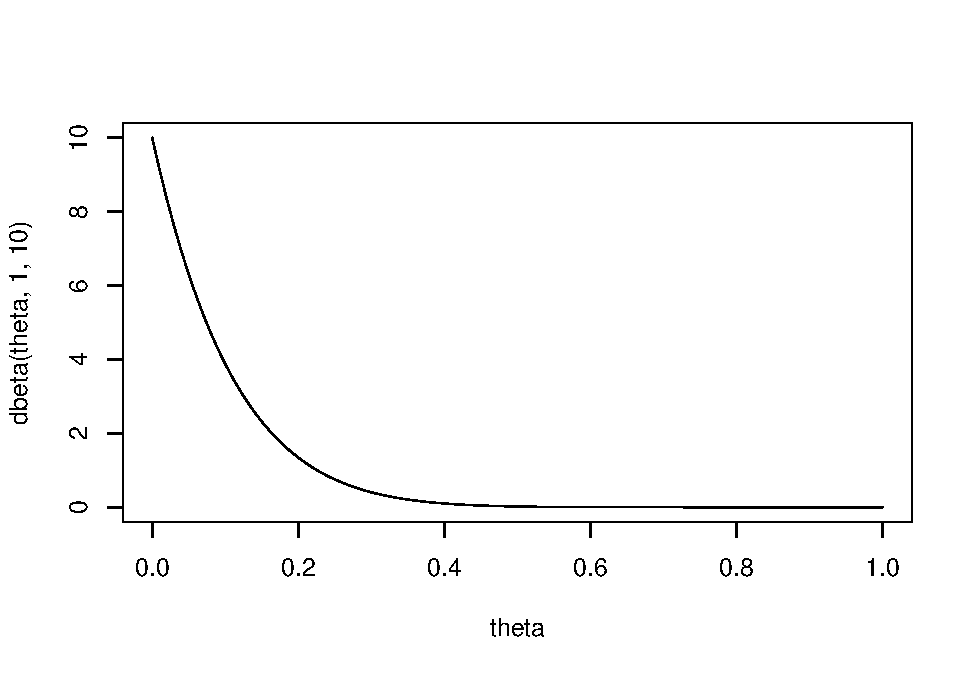
\includegraphics{_main_files/figure-latex/unnamed-chunk-6-1.pdf}

\begin{enumerate}
\def\labelenumi{(\alph{enumi})}
\setcounter{enumi}{1}
\tightlist
\item
  In the period of 1900-1992, there were 20,597 elections, out of which 6 were decided by less than 10 votes, and 49 were decided by less than 100 votes.\\
  we can estimate the probability of a tie to be less than 6/20,597 and bounded by 49/20,597. So for the Binomial trials the sum of the successes is 6, and n=20,597, so the posterior could be \(\theta | y \sim Beta(1+6, 10+20,597 -6)\) is the posterior for \(\theta\). This assumes that 10 votes is within the neighborhood of an election tie.\\
  The question asks to compute at least one election tie, from a total of 435 elections. This follows a Binomial(435, \(\hat{\theta})\). Where we use the posterior mean to estimate \(\theta\). The posterior mean using the Beta(7,20601) yields a mean of \(\hat{\theta}=\frac{7}{20608} = 3.4e-04\) as the posterior mean.
\end{enumerate}

Then the probability that at least 1 election is tied, from 435 total elections will follow a Binomial(435, \(\hat{\theta})\), where we can use the posterior distribution for \(\theta | y\) in the Binomial likelihood \(P(X\geq 1 | \hat{\theta})= 1-P(X\leq0 | \hat{\theta})\) which has a probability of 0.14 of at least 1 election tie.

\begin{Shaded}
\begin{Highlighting}[]
 \CommentTok{\# the posterior for theta is Beta(1+6,10+20597{-}6)}
 \FunctionTok{plot}\NormalTok{(theta,}\FunctionTok{dbeta}\NormalTok{(theta,}\DecValTok{7}\NormalTok{,}\DecValTok{10}\SpecialCharTok{+}\DecValTok{20597{-}6}\NormalTok{),}\AttributeTok{type=}\StringTok{\textquotesingle{}l\textquotesingle{}}\NormalTok{)}
\end{Highlighting}
\end{Shaded}

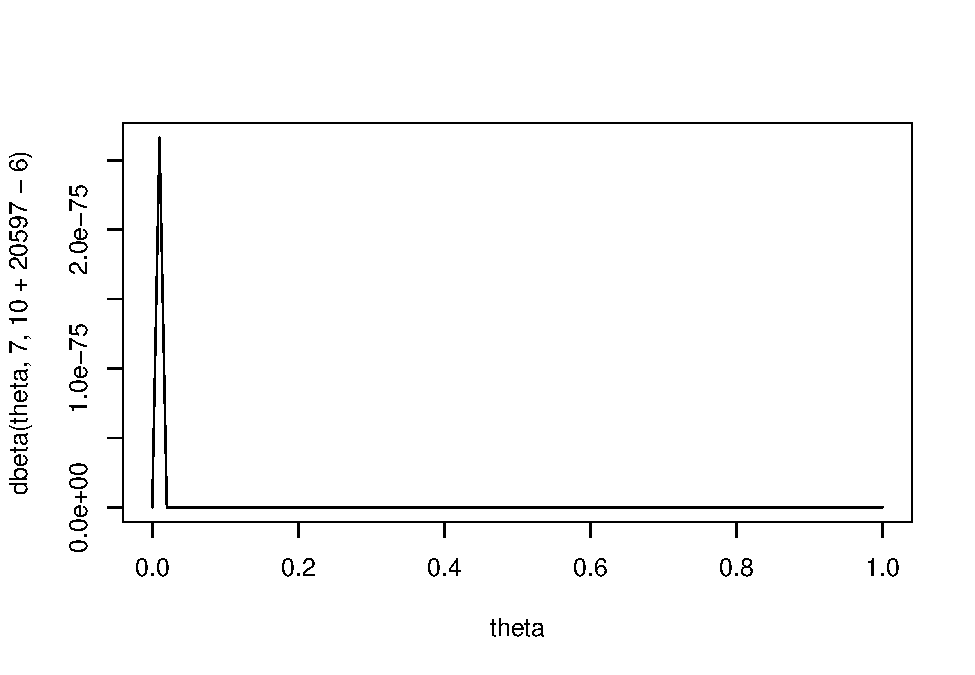
\includegraphics{_main_files/figure-latex/unnamed-chunk-7-1.pdf}

\begin{Shaded}
\begin{Highlighting}[]
 \DocumentationTok{\#\# posterior mean is 7/(20601)}
\DocumentationTok{\#\# then P(X\textgreater{}=1) = 1{-}P(X\textless{}=0 | p)}
  \DecValTok{1}\SpecialCharTok{{-}}\FunctionTok{pbinom}\NormalTok{(}\DecValTok{0}\NormalTok{,}\DecValTok{435}\NormalTok{,}\AttributeTok{prob=}\DecValTok{7}\SpecialCharTok{/}\DecValTok{20608}\NormalTok{)}
\end{Highlighting}
\end{Shaded}

\begin{verbatim}
## [1] 0.1373819
\end{verbatim}

\begin{enumerate}
\def\labelenumi{\arabic{enumi}.}
\setcounter{enumi}{8}
\item
  A clinic has three doctors. Patients come into the clinic at random, starting at 9 a.m. according to a Poisson process, with a time parameter, t, of 10 minutes; that is after opening the first patient appears follows an exponential distribution with average waiting time of 10 minutes. Then the next patient arrives with a waiting time of an expected 10 minutes as iid exponential distribution. After a patient arrives, the patient waits until a doctor is available, and the doctor visits a patitient uniformly between 5-20 minutes. The clinic stops admitting patients at 4 pm, and closes after the last patient is completed with the visit.

  \begin{enumerate}
  \def\labelenumii{(\alph{enumii})}
  \tightlist
  \item
    Simulate this process once. how many patients visited the office? how many had to wait for a doctor? what was the average wait? when did office close?
  \end{enumerate}
\end{enumerate}

\begin{Shaded}
\begin{Highlighting}[]
\DocumentationTok{\#\#\# waiting time for a new patient to arrive in the clinic}
\DocumentationTok{\#\#\#\#\#\#\#\#\#\#\#\#\#\#\#\#\#\#\#\#\#\#\#\#\#\#\#\#\#\#\#\#\#\#\#\#\#\#\#\#\#\#\#\#\#\#\#\#\#\#\#\#\#\#\#\#\#\#\#}
 \CommentTok{\# patientList is the data frame of all patients}
 \CommentTok{\# closeTime is the time to stop admitting (420 minutes)}
 \CommentTok{\# currentPatient Number }
 \CommentTok{\# current time is the running total of time}
\NormalTok{  newPatientArrival}\OtherTok{\textless{}{-}}\ControlFlowTok{function}\NormalTok{(patientList,}
                             \AttributeTok{closeTime=}\NormalTok{timeToClose,}
\NormalTok{                              waitTime,}
\NormalTok{                             visitTime,}
                             \AttributeTok{currentPatientNumber=}\DecValTok{0}\NormalTok{,}
\NormalTok{                             currentTime,}
                             \AttributeTok{assignedDoctor=}\StringTok{"none"}\NormalTok{,}
                             \AttributeTok{completionTime=}\DecValTok{0}\NormalTok{)\{}
    \CommentTok{\# waiting time for next patient}
\NormalTok{     patientTime}\OtherTok{\textless{}{-}}\FunctionTok{round}\NormalTok{(}\FunctionTok{rexp}\NormalTok{(}\DecValTok{1}\NormalTok{,}\AttributeTok{rate=}\DecValTok{1}\SpecialCharTok{/}\DecValTok{10}\NormalTok{),}\DecValTok{2}\NormalTok{)}
    \CommentTok{\# current time of existing patients}
\NormalTok{     current}\OtherTok{\textless{}{-}}\FunctionTok{max}\NormalTok{(patientList}\SpecialCharTok{$}\NormalTok{currentTime)}
   \DocumentationTok{\#\# the clinic stops admitting patients at 4pm}
   \ControlFlowTok{if}\NormalTok{( (current}\SpecialCharTok{+}\NormalTok{patientTime)}\SpecialCharTok{\textless{}=}\NormalTok{closeTime)\{}
     \DocumentationTok{\#\# in minutes}
\NormalTok{   newPatient}\OtherTok{\textless{}{-}}\FunctionTok{createPatientChart}\NormalTok{(currentPatientNumber,patientTime,waitTime,visitTime,currentTime,assignedDoctor,}\DecValTok{0}\NormalTok{)}
\NormalTok{    \}}\ControlFlowTok{else}\NormalTok{\{}
\NormalTok{    newPatient}\OtherTok{\textless{}{-}}\FunctionTok{createPatientChart}\NormalTok{(currentPatientNumber,patientTime,waitTime,visitTime,currentTime,}\StringTok{"closed\_notAdmitted"}\NormalTok{,}\DecValTok{0}\NormalTok{)}
\NormalTok{   \}}
   \FunctionTok{return}\NormalTok{(newPatient)}
\NormalTok{ \}}
\DocumentationTok{\#\#\#\#\#\#\#\#\#\#\#\#\#\#\#\#\#\#\#\# }
 
 
 
\NormalTok{ computeWaitTime}\OtherTok{\textless{}{-}}\ControlFlowTok{function}\NormalTok{(}\AttributeTok{doctors=}\ConstantTok{NULL}\NormalTok{,}
                           \AttributeTok{patientList=}\ConstantTok{NULL}\NormalTok{,}
                           \AttributeTok{patientID=}\DecValTok{1}\NormalTok{)\{}
   \DocumentationTok{\#\# need to compute visiting time (booked)}
   \DocumentationTok{\#\# next time available}
   \DocumentationTok{\#\# required input current time for a specific doctor/patient ?}
   \CommentTok{\# patient time (minutes)}
   
   \DocumentationTok{\#\# FIX ME: it is grabbing 2 patient IDs?}
\NormalTok{   currentTime}\OtherTok{\textless{}{-}}\NormalTok{patientList}\SpecialCharTok{$}\NormalTok{currentTime[}\FunctionTok{which}\NormalTok{(patientList}\SpecialCharTok{$}\NormalTok{patient}\SpecialCharTok{==}\NormalTok{patientID)]}
\NormalTok{   visitTime}\OtherTok{\textless{}{-}}\FunctionTok{runif}\NormalTok{(}\DecValTok{1}\NormalTok{,}\AttributeTok{min=}\DecValTok{5}\NormalTok{,}\AttributeTok{max=}\DecValTok{20}\NormalTok{) }\DocumentationTok{\#\# minutes}
 
   
   \ControlFlowTok{if}\NormalTok{(}\FunctionTok{any}\NormalTok{(doctors}\SpecialCharTok{$}\NormalTok{nextTimeAvail}\SpecialCharTok{\textless{}}\NormalTok{currentTime))\{}
\NormalTok{     waitTime}\OtherTok{=}\DecValTok{0}
\NormalTok{     assignedDr}\OtherTok{\textless{}{-}}\FunctionTok{sample}\NormalTok{(doctors}\SpecialCharTok{$}\NormalTok{dr[}\FunctionTok{which}\NormalTok{(doctors}\SpecialCharTok{$}\NormalTok{nextTimeAvail}\SpecialCharTok{\textless{}}\NormalTok{currentTime)],}\DecValTok{1}\NormalTok{)}
     \DocumentationTok{\#\#\# current time + visitTime}
\NormalTok{     nextAvailTime}\OtherTok{\textless{}{-}}\NormalTok{ visitTime}\SpecialCharTok{+}\NormalTok{currentTime}\SpecialCharTok{+}\NormalTok{waitTime}
     \DocumentationTok{\#\# completion time for patient exit (closing time).}
\NormalTok{   \}}\ControlFlowTok{else} \ControlFlowTok{if}\NormalTok{(}\FunctionTok{any}\NormalTok{(doctors}\SpecialCharTok{$}\NormalTok{nextTimeAvail}\SpecialCharTok{\textless{}}\NormalTok{currentTime)}\SpecialCharTok{==}\ConstantTok{FALSE}\NormalTok{)\{}
     \CommentTok{\# all doctors are booked, no available doctors.}
     \CommentTok{\# wait time is the difference between next available time (assuming all times are greater than patient time)}
\NormalTok{     waitTime}\OtherTok{\textless{}{-}}\FunctionTok{min}\NormalTok{(doctors}\SpecialCharTok{$}\NormalTok{nextTimeAvail}\SpecialCharTok{{-}}\NormalTok{currentTime)}
\NormalTok{     assignedDr}\OtherTok{\textless{}{-}}\NormalTok{doctors}\SpecialCharTok{$}\NormalTok{dr[}\FunctionTok{which}\NormalTok{( (doctors}\SpecialCharTok{$}\NormalTok{nextTimeAvail}\SpecialCharTok{{-}}\NormalTok{currentTime)}\SpecialCharTok{==}\FunctionTok{min}\NormalTok{(doctors}\SpecialCharTok{$}\NormalTok{nextTimeAvail}\SpecialCharTok{{-}}\NormalTok{currentTime))]}
       \ControlFlowTok{if}\NormalTok{(}\FunctionTok{length}\NormalTok{(assignedDr)}\SpecialCharTok{\textgreater{}}\DecValTok{1}\NormalTok{)\{}
\NormalTok{         assignedDr}\OtherTok{\textless{}{-}}\NormalTok{assignedDr[}\DecValTok{1}\NormalTok{]}
\NormalTok{       \}}
\NormalTok{     nextAvailTime}\OtherTok{\textless{}{-}}\NormalTok{ visitTime}\SpecialCharTok{+}\NormalTok{currentTime}\SpecialCharTok{+}\NormalTok{waitTime  }\DocumentationTok{\#\# completion time for patient to exit}
\NormalTok{    \}}\DocumentationTok{\#\# if all doctors unavail}
    \CommentTok{\#print(assignedDr)}
    \CommentTok{\#print(currentTime)}
    \DocumentationTok{\#\#  update doctor list}
\NormalTok{     doctors[}\FunctionTok{which}\NormalTok{(doctors}\SpecialCharTok{$}\NormalTok{dr}\SpecialCharTok{==}\NormalTok{assignedDr),}\StringTok{\textquotesingle{}visitingPatient\textquotesingle{}}\NormalTok{]}\OtherTok{\textless{}{-}}\NormalTok{patientID}
\NormalTok{     doctors[}\FunctionTok{which}\NormalTok{(doctors}\SpecialCharTok{$}\NormalTok{dr}\SpecialCharTok{==}\NormalTok{assignedDr),}\StringTok{\textquotesingle{}nextTimeAvail\textquotesingle{}}\NormalTok{]}\OtherTok{\textless{}{-}}\NormalTok{nextAvailTime}
\NormalTok{     doctors[}\FunctionTok{which}\NormalTok{(doctors}\SpecialCharTok{$}\NormalTok{dr}\SpecialCharTok{==}\NormalTok{assignedDr),}\StringTok{\textquotesingle{}currentTime\textquotesingle{}}\NormalTok{]}\OtherTok{\textless{}{-}}\NormalTok{currentTime }\DocumentationTok{\#\# patient time}
\NormalTok{     doctors[}\FunctionTok{which}\NormalTok{(doctors}\SpecialCharTok{$}\NormalTok{dr}\SpecialCharTok{==}\NormalTok{assignedDr),}\StringTok{\textquotesingle{}visitTimeLength\textquotesingle{}}\NormalTok{]}\OtherTok{\textless{}{-}}\NormalTok{visitTime}
     \CommentTok{\# flag avail to no.}
\NormalTok{     doctors[}\FunctionTok{which}\NormalTok{(doctors}\SpecialCharTok{$}\NormalTok{dr}\SpecialCharTok{==}\NormalTok{assignedDr),}\StringTok{\textquotesingle{}avail\textquotesingle{}}\NormalTok{]}\OtherTok{\textless{}{-}}\StringTok{\textquotesingle{}no\textquotesingle{}}
     \DocumentationTok{\#\# update patient list}
\NormalTok{     patientList[}\FunctionTok{which}\NormalTok{(patientList}\SpecialCharTok{$}\NormalTok{patient}\SpecialCharTok{==}\NormalTok{patientID),}\StringTok{\textquotesingle{}doctorWaitTime\textquotesingle{}}\NormalTok{]}\OtherTok{\textless{}{-}}\NormalTok{waitTime}
\NormalTok{     patientList[}\FunctionTok{which}\NormalTok{(patientList}\SpecialCharTok{$}\NormalTok{patient}\SpecialCharTok{==}\NormalTok{patientID),}\StringTok{\textquotesingle{}doctorVisitTime\textquotesingle{}}\NormalTok{]}\OtherTok{\textless{}{-}}\NormalTok{visitTime}
\NormalTok{     patientList[}\FunctionTok{which}\NormalTok{(patientList}\SpecialCharTok{$}\NormalTok{patient}\SpecialCharTok{==}\NormalTok{patientID),}\StringTok{\textquotesingle{}assignedDoctor\textquotesingle{}}\NormalTok{]}\OtherTok{\textless{}{-}}\NormalTok{assignedDr}
\NormalTok{     patientList[}\FunctionTok{which}\NormalTok{(patientList}\SpecialCharTok{$}\NormalTok{patient}\SpecialCharTok{==}\NormalTok{patientID),}\StringTok{\textquotesingle{}completionTime\textquotesingle{}}\NormalTok{]}\OtherTok{\textless{}{-}}\NormalTok{nextAvailTime}
   \FunctionTok{return}\NormalTok{(}\FunctionTok{list}\NormalTok{(}\AttributeTok{patient=}\NormalTok{patientList,}\AttributeTok{doctor=}\NormalTok{doctors))}
\NormalTok{ \}}
 
 
 \DocumentationTok{\#\# creates a patient object}
\NormalTok{ createPatientChart}\OtherTok{\textless{}{-}}\ControlFlowTok{function}\NormalTok{(currentPatientNumber,arrivalTime,waitTime,visitTime,currentTime,assignedDoctor,completionTime)\{}
\NormalTok{   patientID}\OtherTok{\textless{}{-}}\FunctionTok{data.frame}\NormalTok{(}\AttributeTok{patient=}\NormalTok{currentPatientNumber}\SpecialCharTok{+}\DecValTok{1}\NormalTok{,}
                         \AttributeTok{arrivalTime=}\NormalTok{arrivalTime,}
                         \AttributeTok{doctorWaitTime=}\NormalTok{waitTime,}
                         \AttributeTok{doctorVisitTime=}\NormalTok{visitTime,}
                         \AttributeTok{currentTime=}\NormalTok{currentTime,}
                         \AttributeTok{assignedDoctor=}\NormalTok{assignedDoctor,}
                         \AttributeTok{completionTime=}\DecValTok{0}\NormalTok{)}
   \FunctionTok{return}\NormalTok{(patientID)}
\NormalTok{ \}}
 
\NormalTok{ updatePatientList}\OtherTok{\textless{}{-}}\ControlFlowTok{function}\NormalTok{(patientList,patientID)\{}
\NormalTok{   patientList}\OtherTok{\textless{}{-}}\FunctionTok{rbind}\NormalTok{(patientList,patientID)}
   \FunctionTok{return}\NormalTok{(patientList)}
\NormalTok{ \}}
 
\NormalTok{updateTime}\OtherTok{\textless{}{-}}\ControlFlowTok{function}\NormalTok{(currentTime,}\AttributeTok{newTime=}\ConstantTok{NULL}\NormalTok{,p1)\{}
\NormalTok{  p1}\SpecialCharTok{$}\NormalTok{currentTime}\OtherTok{\textless{}{-}}\NormalTok{currentTime}\SpecialCharTok{+}\NormalTok{newTime}
  \FunctionTok{return}\NormalTok{(p1)}
\NormalTok{\}}
\NormalTok{ totalPatients}\OtherTok{\textless{}{-}}\DecValTok{0}
\DocumentationTok{\#\# this is the simulation}
 \DocumentationTok{\#\# first task : loop through the time update for patients}
 \DocumentationTok{\#\# second task : include the doctor assignment query.}
\NormalTok{simulateProcess}\OtherTok{\textless{}{-}}\ControlFlowTok{function}\NormalTok{(}\AttributeTok{doctors=}\ConstantTok{NULL}\NormalTok{,}
                          \AttributeTok{totalWait=}\ConstantTok{NULL}\NormalTok{,}
                          \AttributeTok{totalPatients=}\DecValTok{0}\NormalTok{,}
                          \AttributeTok{timeToClose=}\DecValTok{420}\NormalTok{,}
                          \AttributeTok{currentTime=}\ConstantTok{NULL}\NormalTok{)\{}
  \DocumentationTok{\#\# initiate Patient List}
\NormalTok{ patientList}\OtherTok{\textless{}{-}}\FunctionTok{data.frame}\NormalTok{(}\AttributeTok{patient=}\DecValTok{0}\NormalTok{,}
                         \AttributeTok{arrivalTime=}\DecValTok{0}\NormalTok{,}
                         \AttributeTok{doctorWaitTime=}\DecValTok{0}\NormalTok{,}
                         \AttributeTok{doctorVisitTime=}\DecValTok{0}\NormalTok{,}
                         \AttributeTok{currentTime=}\DecValTok{0}\NormalTok{,}
                         \AttributeTok{assignedDoctor=}\StringTok{\textquotesingle{}none\textquotesingle{}}\NormalTok{,}
                         \AttributeTok{completionTime=}\DecValTok{0}\NormalTok{)}
 \DocumentationTok{\#\# not sure what to put here.}
\NormalTok{ currentTime}\OtherTok{\textless{}{-}}\NormalTok{patientList}\SpecialCharTok{$}\NormalTok{currentTime[}\FunctionTok{which}\NormalTok{(patientList}\SpecialCharTok{$}\NormalTok{patient}\SpecialCharTok{==}\FunctionTok{max}\NormalTok{(patientList}\SpecialCharTok{$}\NormalTok{patient))] }\DocumentationTok{\#\# current time is the max current time from patient chart.}
\NormalTok{ currentPatientNumber}\OtherTok{\textless{}{-}}\DecValTok{0}
 
 \DocumentationTok{\#\# timeToClose (minutes) is stopping to admit patients}
  \ControlFlowTok{while}\NormalTok{(currentTime}\SpecialCharTok{\textless{}}\NormalTok{timeToClose)\{}
    \DocumentationTok{\#\# patient enters after the (i{-}1) patient enters.}
\NormalTok{    p1}\OtherTok{\textless{}{-}}\FunctionTok{newPatientArrival}\NormalTok{(patientList,}
                             \AttributeTok{closeTime=}\NormalTok{timeToClose,}
                          \AttributeTok{waitTime=}\DecValTok{0}\NormalTok{,}
                          \AttributeTok{visitTime=}\DecValTok{0}\NormalTok{,}
                             \AttributeTok{currentPatientNumber=}\NormalTok{currentPatientNumber,}
\NormalTok{                             currentTime)}
    \DocumentationTok{\#\# update time}
\NormalTok{    p1}\OtherTok{\textless{}{-}}\FunctionTok{updateTime}\NormalTok{(p1}\SpecialCharTok{$}\NormalTok{currentTime,}\AttributeTok{newTime=}\NormalTok{p1}\SpecialCharTok{$}\NormalTok{arrivalTime,p1)}
    
    \CommentTok{\# given a patient time, switch the availability of any doctor}
    \CommentTok{\# if a doctors next available time is less than the current time, switch him to available}
    \DocumentationTok{\#\# FIX ME: need to ensure this flag is correct.}
    \ControlFlowTok{if}\NormalTok{(}\FunctionTok{any}\NormalTok{(doctors}\SpecialCharTok{$}\NormalTok{nextTimeAvail}\SpecialCharTok{\textless{}}\NormalTok{p1}\SpecialCharTok{$}\NormalTok{currentTime))\{}
\NormalTok{      doctors}\SpecialCharTok{$}\NormalTok{avail[}\FunctionTok{which}\NormalTok{(doctors}\SpecialCharTok{$}\NormalTok{nextTimeAvail}\SpecialCharTok{\textless{}}\NormalTok{p1}\SpecialCharTok{$}\NormalTok{currentTime)]}\OtherTok{\textless{}{-}}\StringTok{\textquotesingle{}yes\textquotesingle{}}
\NormalTok{    \}}
    
    \DocumentationTok{\#\# create a patient list}
    \ControlFlowTok{if}\NormalTok{(currentPatientNumber}\SpecialCharTok{==}\DecValTok{0}\NormalTok{)\{}
\NormalTok{      patientList}\OtherTok{\textless{}{-}}\NormalTok{p1}
     \CommentTok{\# update patient number  }
\NormalTok{      currentPatientNumber}\OtherTok{\textless{}{-}}\NormalTok{currentPatientNumber}\SpecialCharTok{+}\DecValTok{1}
\NormalTok{    \}}\ControlFlowTok{else}\NormalTok{\{}
\NormalTok{      patientList}\OtherTok{\textless{}{-}}\FunctionTok{rbind}\NormalTok{(patientList,p1)}
     \CommentTok{\# update patient number  }
\NormalTok{      currentPatientNumber}\OtherTok{\textless{}{-}}\NormalTok{currentPatientNumber}\SpecialCharTok{+}\DecValTok{1}
\NormalTok{    \}}
    
    \DocumentationTok{\#\# task 2 assign a doctor}
     \DocumentationTok{\#\#\# check for doctor availability}
     \DocumentationTok{\#\# compute wait time, and/or compute the next available time}
     \DocumentationTok{\#\# returns a list object.}
\NormalTok{    clinicList}\OtherTok{\textless{}{-}}\FunctionTok{computeWaitTime}\NormalTok{(doctors,patientList,}\AttributeTok{patientID=}\NormalTok{patientList}\SpecialCharTok{$}\NormalTok{patient[currentPatientNumber])}
  
\NormalTok{    doctors}\OtherTok{\textless{}{-}}\NormalTok{clinicList[[}\StringTok{"doctor"}\NormalTok{]]}
\NormalTok{   patientList}\OtherTok{\textless{}{-}}\NormalTok{clinicList[[}\StringTok{"patient"}\NormalTok{]]}
   \DocumentationTok{\#\# update flags}
     \CommentTok{\# update currentTime}
    \DocumentationTok{\#\# current time is cumulative sum of the arrival times.}
\NormalTok{   currentTime}\OtherTok{\textless{}{-}}\NormalTok{patientList}\SpecialCharTok{$}\NormalTok{currentTime[}\FunctionTok{which}\NormalTok{(patientList}\SpecialCharTok{$}\NormalTok{patient}\SpecialCharTok{==}\FunctionTok{max}\NormalTok{(patientList}\SpecialCharTok{$}\NormalTok{patient))] }\DocumentationTok{\#\# current time is the max current time from patient chart.}
   
   \DocumentationTok{\#\# fix me:}
   \DocumentationTok{\#\# reset doctor availability based on current patient time.}
\NormalTok{   upID}\OtherTok{\textless{}{-}}\FunctionTok{which}\NormalTok{(doctors}\SpecialCharTok{$}\NormalTok{nextTimeAvail}\SpecialCharTok{\textless{}}\NormalTok{currentTime)}
\NormalTok{   doctors}\SpecialCharTok{$}\NormalTok{nextTimeAvail[upID]}\OtherTok{\textless{}{-}}\NormalTok{currentTime}
\NormalTok{   doctors}\SpecialCharTok{$}\NormalTok{currentTime[upID]}\OtherTok{\textless{}{-}}\NormalTok{currentTime }
\NormalTok{   doctors}\SpecialCharTok{$}\NormalTok{visitTimeLength[upID]}\OtherTok{\textless{}{-}}\DecValTok{0} 
\NormalTok{  \}}\DocumentationTok{\#\# while loop}
  \FunctionTok{return}\NormalTok{(}\FunctionTok{list}\NormalTok{(}\AttributeTok{patient=}\NormalTok{patientList,}\AttributeTok{doctors=}\NormalTok{doctors))}
\NormalTok{\}}
\end{Highlighting}
\end{Shaded}

\begin{Shaded}
\begin{Highlighting}[]
\NormalTok{ doctors}\OtherTok{\textless{}{-}}\FunctionTok{data.frame}\NormalTok{(}\AttributeTok{dr=}\FunctionTok{c}\NormalTok{(}\StringTok{\textquotesingle{}a\textquotesingle{}}\NormalTok{,}\StringTok{\textquotesingle{}b\textquotesingle{}}\NormalTok{,}\StringTok{\textquotesingle{}c\textquotesingle{}}\NormalTok{),}
                     \AttributeTok{visitingPatient=}\FunctionTok{c}\NormalTok{(}\DecValTok{0}\NormalTok{,}\DecValTok{0}\NormalTok{,}\DecValTok{0}\NormalTok{), }\DocumentationTok{\#\# who is doctor seeing (patient ID)}
                     \AttributeTok{visitTimeLength=}\FunctionTok{c}\NormalTok{(}\DecValTok{0}\NormalTok{,}\DecValTok{0}\NormalTok{,}\DecValTok{0}\NormalTok{), }\CommentTok{\# length of doctor visit U(5,20)}
                     \AttributeTok{currentTime=}\FunctionTok{c}\NormalTok{(}\DecValTok{0}\NormalTok{,}\DecValTok{0}\NormalTok{,}\DecValTok{0}\NormalTok{),    }\DocumentationTok{\#\# current Time}
                     \AttributeTok{nextTimeAvail=}\FunctionTok{c}\NormalTok{(}\DecValTok{0}\NormalTok{,}\DecValTok{0}\NormalTok{,}\DecValTok{0}\NormalTok{),  }\DocumentationTok{\#\# current time + visitTimeLength = next avail time.}
                     \AttributeTok{avail=}\FunctionTok{c}\NormalTok{(}\StringTok{"yes"}\NormalTok{,}\StringTok{"yes"}\NormalTok{,}\StringTok{"yes"}\NormalTok{))}
\DocumentationTok{\#\# initiate times}
\NormalTok{ totalWait}\OtherTok{\textless{}{-}}\DecValTok{0}
\NormalTok{ currentPatientNumber}\OtherTok{\textless{}{-}}\DecValTok{0}
 \DocumentationTok{\#\# clinic opens at 9am {-}4pm that is 7 hours (420 min.)}
\NormalTok{ timeToClose}\OtherTok{\textless{}{-}}\DecValTok{7}\SpecialCharTok{*}\DecValTok{60} \DocumentationTok{\#\# stops admiting patienets in 420 minutes}
 \DocumentationTok{\#\# current time is 0}
 \DocumentationTok{\#\# this will be the running total of minutes.}
\NormalTok{ currentTime}\OtherTok{\textless{}{-}}\DecValTok{0}
 
 
 
\NormalTok{res}\OtherTok{\textless{}{-}}\FunctionTok{simulateProcess}\NormalTok{(doctors,}
\NormalTok{                          totalWait,}
\NormalTok{                          totalPatients,}
\NormalTok{                          timeToClose,}
\NormalTok{                          currentTime)}

\NormalTok{pl}\OtherTok{\textless{}{-}}\NormalTok{res}\SpecialCharTok{$}\NormalTok{patient[}\FunctionTok{which}\NormalTok{(res}\SpecialCharTok{$}\NormalTok{patient}\SpecialCharTok{$}\NormalTok{currentTime}\SpecialCharTok{\textless{}=}\DecValTok{420}\NormalTok{),]}

 \FunctionTok{hist}\NormalTok{(pl}\SpecialCharTok{$}\NormalTok{doctorVisitTime)}
 \FunctionTok{abline}\NormalTok{(}\AttributeTok{v=}\NormalTok{(}\DecValTok{20}\SpecialCharTok{+}\DecValTok{5}\NormalTok{)}\SpecialCharTok{/}\DecValTok{2}\NormalTok{) }\DocumentationTok{\#\# should be \textasciitilde{}12}
\end{Highlighting}
\end{Shaded}

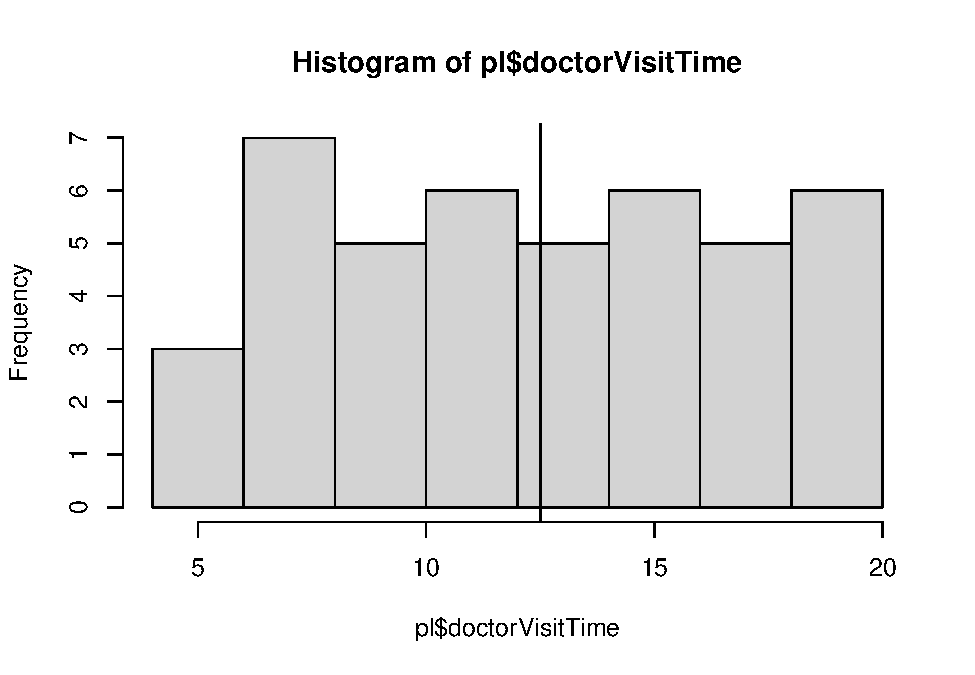
\includegraphics{_main_files/figure-latex/unnamed-chunk-9-1.pdf}

\begin{Shaded}
\begin{Highlighting}[]
 \FunctionTok{hist}\NormalTok{(pl}\SpecialCharTok{$}\NormalTok{arrivalTime) }\DocumentationTok{\#\# should be close to 10  exp(1/10) has mean 10}
\end{Highlighting}
\end{Shaded}

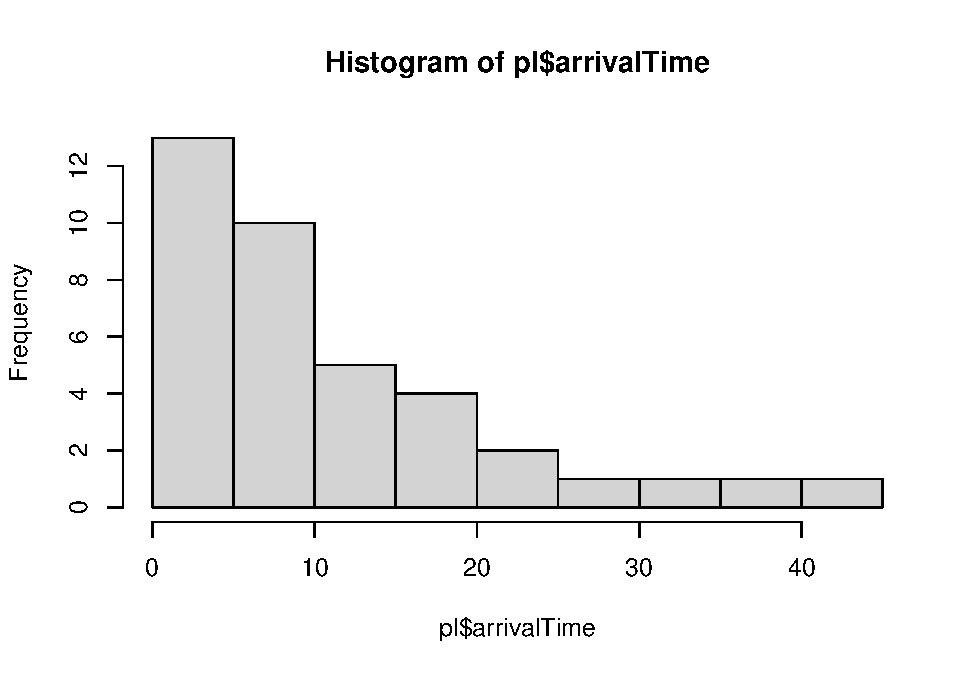
\includegraphics{_main_files/figure-latex/unnamed-chunk-9-2.pdf}

\begin{Shaded}
\begin{Highlighting}[]
  \FunctionTok{hist}\NormalTok{(pl}\SpecialCharTok{$}\NormalTok{doctorWaitTime[}\FunctionTok{which}\NormalTok{(pl}\SpecialCharTok{$}\NormalTok{doctorWaitTime}\SpecialCharTok{!=}\DecValTok{0}\NormalTok{)]) }\DocumentationTok{\#\# about 2.41}
\end{Highlighting}
\end{Shaded}

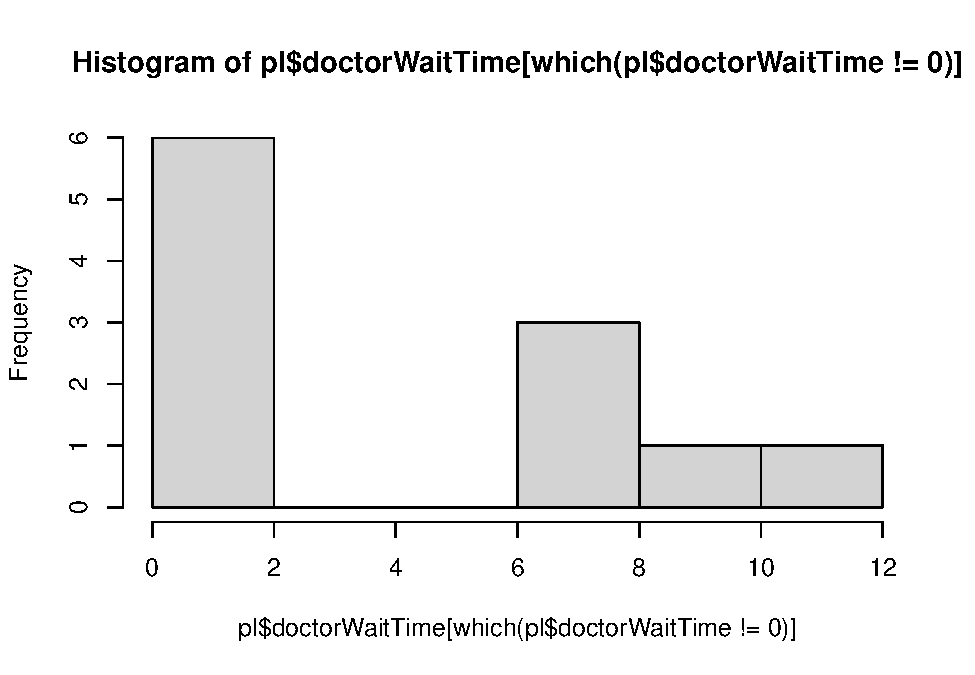
\includegraphics{_main_files/figure-latex/unnamed-chunk-9-3.pdf}

\begin{Shaded}
\begin{Highlighting}[]
  \FunctionTok{print}\NormalTok{(}\FunctionTok{max}\NormalTok{(pl}\SpecialCharTok{$}\NormalTok{completionTime)}\SpecialCharTok{{-}}\DecValTok{420}\NormalTok{) }\DocumentationTok{\#\# closing time}
\end{Highlighting}
\end{Shaded}

\begin{verbatim}
## [1] -0.4080558
\end{verbatim}

\begin{Shaded}
\begin{Highlighting}[]
  \FunctionTok{print}\NormalTok{(}\FunctionTok{max}\NormalTok{(pl}\SpecialCharTok{$}\NormalTok{patient)) }\DocumentationTok{\#\# total patient  should be 42}
\end{Highlighting}
\end{Shaded}

\begin{verbatim}
## [1] 38
\end{verbatim}

\begin{Shaded}
\begin{Highlighting}[]
\DocumentationTok{\#\# (20{-}5)/6 + 10 this is about 12.5 minutes of arrival + visit time. which is approximately close to 10 }
\DocumentationTok{\#\# the arrival time is about 10 minutes.  }

\DocumentationTok{\#\# we should expect 42 patients}
 \CommentTok{\#420/10}
  
  \DocumentationTok{\#\# sanity check}
  \CommentTok{\#all(pl$currentTime+pl$doctorWaitTime+pl$doctorVisitTime{-}pl$completionTime==0)}
\end{Highlighting}
\end{Shaded}

\hypertarget{simulation-100-times}{%
\section*{Simulation 100 times}\label{simulation-100-times}}
\addcontentsline{toc}{section}{Simulation 100 times}

total number of patients was approximately 42, which we expect since the total 420/10. The total number waiting with 3 doctors is 6.61 for 1 day. the average waiting time was about 4-5 minutes. For 1 day, the average closing time was 5.32 minutes after 4 pm

\begin{Shaded}
\begin{Highlighting}[]
\NormalTok{ totalPat}\OtherTok{\textless{}{-}}\ConstantTok{NULL}
\NormalTok{ totalWaiting}\OtherTok{\textless{}{-}}\ConstantTok{NULL}
\NormalTok{ avgWaiting}\OtherTok{\textless{}{-}}\ConstantTok{NULL}
\NormalTok{ closing}\OtherTok{\textless{}{-}}\ConstantTok{NULL}
\NormalTok{ patientList}\OtherTok{\textless{}{-}}\ConstantTok{NULL}
\NormalTok{ p1}\OtherTok{\textless{}{-}}\ConstantTok{NULL}
 
\ControlFlowTok{for}\NormalTok{(i }\ControlFlowTok{in} \DecValTok{1}\SpecialCharTok{:}\DecValTok{100}\NormalTok{)\{}
  
\NormalTok{ doctors}\OtherTok{\textless{}{-}}\FunctionTok{data.frame}\NormalTok{(}\AttributeTok{dr=}\FunctionTok{c}\NormalTok{(}\StringTok{\textquotesingle{}a\textquotesingle{}}\NormalTok{,}\StringTok{\textquotesingle{}b\textquotesingle{}}\NormalTok{,}\StringTok{\textquotesingle{}c\textquotesingle{}}\NormalTok{),}
                     \AttributeTok{visitingPatient=}\FunctionTok{c}\NormalTok{(}\DecValTok{0}\NormalTok{,}\DecValTok{0}\NormalTok{,}\DecValTok{0}\NormalTok{), }\DocumentationTok{\#\# who is doctor seeing (patient ID)}
                     \AttributeTok{visitTimeLength=}\FunctionTok{c}\NormalTok{(}\DecValTok{0}\NormalTok{,}\DecValTok{0}\NormalTok{,}\DecValTok{0}\NormalTok{), }\CommentTok{\# length of doctor visit U(5,20)}
                     \AttributeTok{currentTime=}\FunctionTok{c}\NormalTok{(}\DecValTok{0}\NormalTok{,}\DecValTok{0}\NormalTok{,}\DecValTok{0}\NormalTok{),    }\DocumentationTok{\#\# current Time}
                     \AttributeTok{nextTimeAvail=}\FunctionTok{c}\NormalTok{(}\DecValTok{0}\NormalTok{,}\DecValTok{0}\NormalTok{,}\DecValTok{0}\NormalTok{),  }\DocumentationTok{\#\# current time + visitTimeLength = next avail time.}
                     \AttributeTok{avail=}\FunctionTok{c}\NormalTok{(}\StringTok{"yes"}\NormalTok{,}\StringTok{"yes"}\NormalTok{,}\StringTok{"yes"}\NormalTok{))}
\DocumentationTok{\#\# initiate times}
\NormalTok{ totalWait}\OtherTok{\textless{}{-}}\DecValTok{0}
\NormalTok{ totalPatients}\OtherTok{\textless{}{-}}\DecValTok{0}
\NormalTok{ currentPatientNumber}\OtherTok{\textless{}{-}}\DecValTok{0}
 \DocumentationTok{\#\# clinic opens at 9am {-}4pm that is 7 hours (420 min.)}
\NormalTok{ timeToClose}\OtherTok{\textless{}{-}}\DecValTok{7}\SpecialCharTok{*}\DecValTok{60} \DocumentationTok{\#\# stops admiting patienets in 420 minutes}
 \DocumentationTok{\#\# current time is 0}
 \DocumentationTok{\#\# this will be the running total of minutes.}
\NormalTok{ currentTime}\OtherTok{\textless{}{-}}\DecValTok{0}
 
 
\NormalTok{res}\OtherTok{\textless{}{-}}\FunctionTok{simulateProcess}\NormalTok{(doctors,}
\NormalTok{                          totalWait,}
\NormalTok{                          totalPatients,}
\NormalTok{                          timeToClose,}
\NormalTok{                          currentTime)}

\NormalTok{pl}\OtherTok{\textless{}{-}}\NormalTok{res}\SpecialCharTok{$}\NormalTok{patient[}\FunctionTok{which}\NormalTok{(res}\SpecialCharTok{$}\NormalTok{patient}\SpecialCharTok{$}\NormalTok{currentTime}\SpecialCharTok{\textless{}=}\DecValTok{420}\NormalTok{),]}


\NormalTok{ totalPat}\OtherTok{\textless{}{-}}\FunctionTok{c}\NormalTok{(totalPat,}\FunctionTok{max}\NormalTok{(pl}\SpecialCharTok{$}\NormalTok{patient))}
\NormalTok{  totalWaiting}\OtherTok{\textless{}{-}}\FunctionTok{c}\NormalTok{(totalWaiting,}\FunctionTok{nrow}\NormalTok{(pl[}\FunctionTok{which}\NormalTok{(pl}\SpecialCharTok{$}\NormalTok{doctorWaitTime}\SpecialCharTok{!=}\DecValTok{0}\NormalTok{),]))}
\NormalTok{ avgWaiting}\OtherTok{\textless{}{-}}\FunctionTok{c}\NormalTok{(avgWaiting,}\FunctionTok{mean}\NormalTok{(pl[}\FunctionTok{which}\NormalTok{(pl}\SpecialCharTok{$}\NormalTok{doctorWaitTime}\SpecialCharTok{!=}\DecValTok{0}\NormalTok{),}\StringTok{"doctorWaitTime"}\NormalTok{]))}
\NormalTok{ closing}\OtherTok{\textless{}{-}}\FunctionTok{c}\NormalTok{(closing,}\FunctionTok{max}\NormalTok{(pl}\SpecialCharTok{$}\NormalTok{completionTime))}
 
\NormalTok{\}}
 
 \FunctionTok{hist}\NormalTok{(totalPat,}\AttributeTok{main=}\StringTok{"total patients"}\NormalTok{)}
 \FunctionTok{abline}\NormalTok{(}\AttributeTok{v=}\DecValTok{420}\SpecialCharTok{/}\DecValTok{10}\NormalTok{,}\AttributeTok{col=}\StringTok{\textquotesingle{}red\textquotesingle{}}\NormalTok{)}
\end{Highlighting}
\end{Shaded}

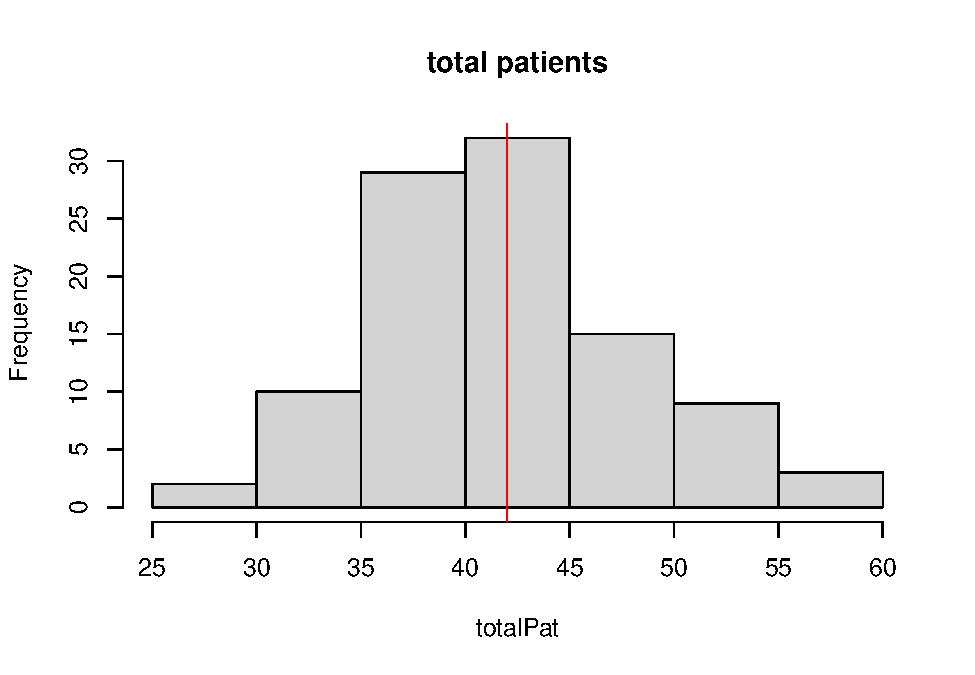
\includegraphics{_main_files/figure-latex/simul-1.pdf}

\begin{Shaded}
\begin{Highlighting}[]
 \FunctionTok{hist}\NormalTok{(totalWaiting,}\AttributeTok{main=}\StringTok{"total number waiting"}\NormalTok{)}
\end{Highlighting}
\end{Shaded}

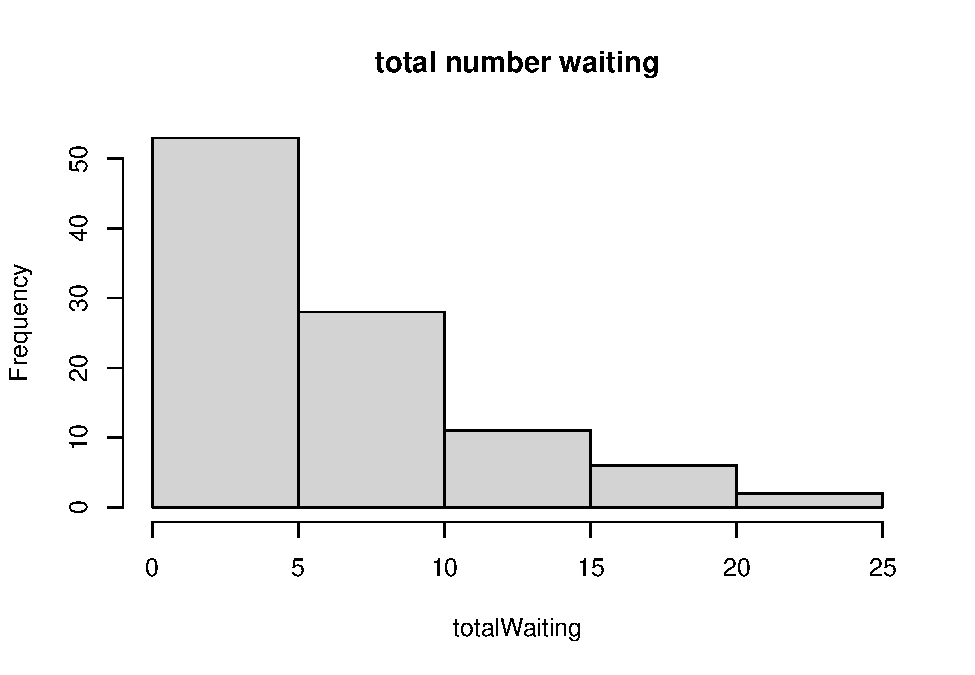
\includegraphics{_main_files/figure-latex/simul-2.pdf}

\begin{Shaded}
\begin{Highlighting}[]
 \FunctionTok{hist}\NormalTok{(avgWaiting,}\AttributeTok{main=}\StringTok{"avg. waiting (min)"}\NormalTok{)}
\end{Highlighting}
\end{Shaded}

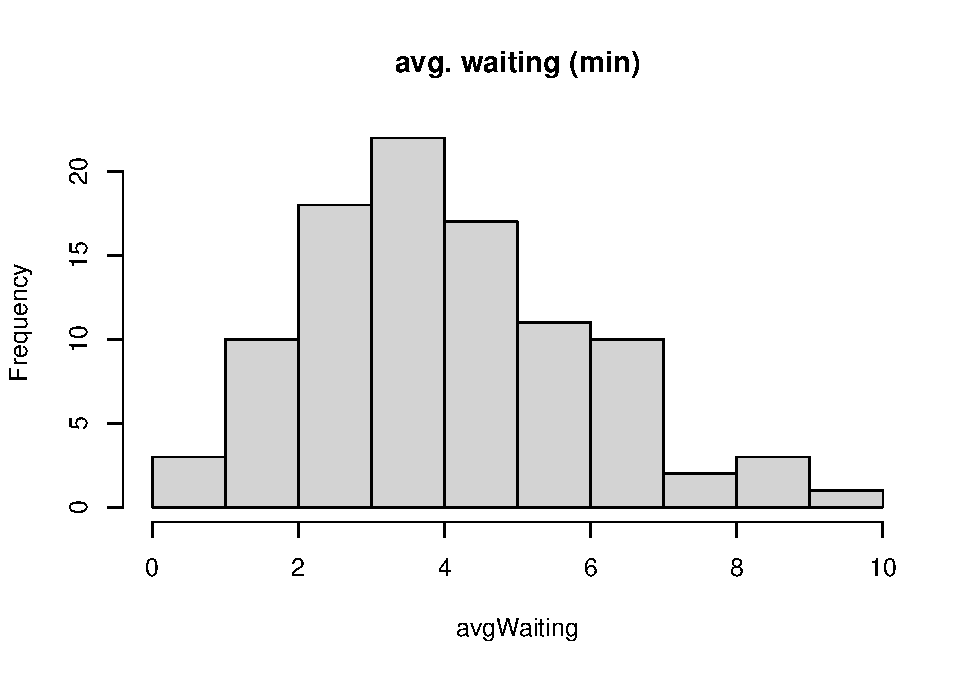
\includegraphics{_main_files/figure-latex/simul-3.pdf}

\begin{Shaded}
\begin{Highlighting}[]
 \FunctionTok{hist}\NormalTok{(closing}\DecValTok{{-}420}\NormalTok{,}\AttributeTok{main=}\StringTok{"closing time"}\NormalTok{)}
\end{Highlighting}
\end{Shaded}

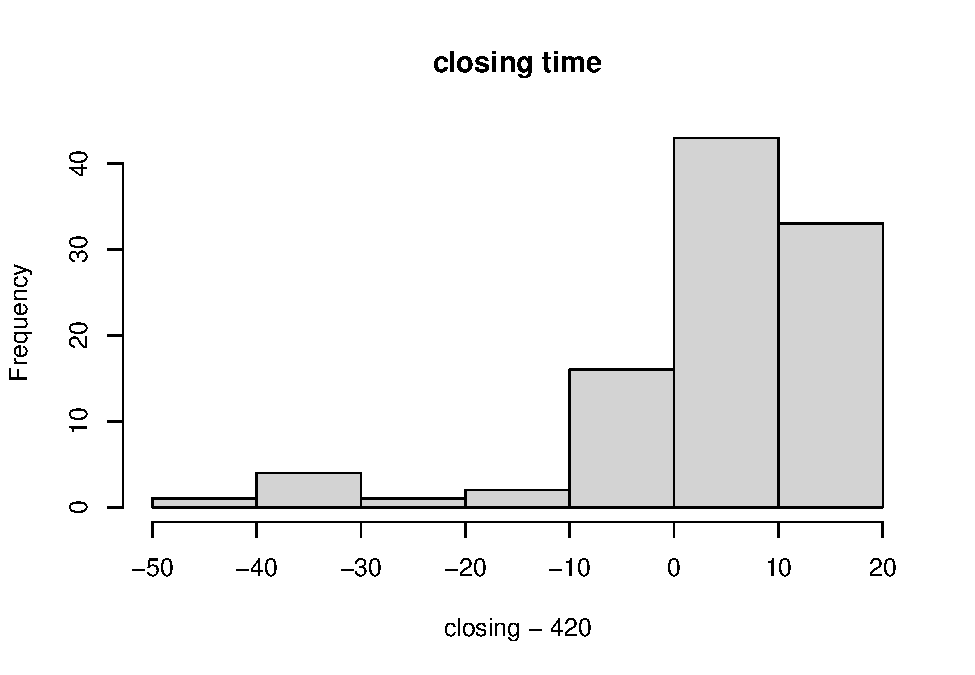
\includegraphics{_main_files/figure-latex/simul-4.pdf}

\hypertarget{cross}{%
\chapter{Single parameter models}\label{cross}}

Cross-references make it easier for your readers to find and link to elements in your book.

\hypertarget{chapters-and-sub-chapters}{%
\section{Chapters and sub-chapters}\label{chapters-and-sub-chapters}}

There are two steps to cross-reference any heading:

\begin{enumerate}
\def\labelenumi{\arabic{enumi}.}
\tightlist
\item
  Label the heading: \texttt{\#\ Hello\ world\ \{\#nice-label\}}.

  \begin{itemize}
  \tightlist
  \item
    Leave the label off if you like the automated heading generated based on your heading title: for example, \texttt{\#\ Hello\ world} = \texttt{\#\ Hello\ world\ \{\#hello-world\}}.
  \item
    To label an un-numbered heading, use: \texttt{\#\ Hello\ world\ \{-\#nice-label\}} or \texttt{\{\#\ Hello\ world\ .unnumbered\}}.
  \end{itemize}
\item
  Next, reference the labeled heading anywhere in the text using \texttt{\textbackslash{}@ref(nice-label)}; for example, please see Chapter \ref{cross}.

  \begin{itemize}
  \tightlist
  \item
    If you prefer text as the link instead of a numbered reference use: \protect\hyperlink{cross}{any text you want can go here}.
  \end{itemize}
\end{enumerate}

\hypertarget{captioned-figures-and-tables}{%
\section{Captioned figures and tables}\label{captioned-figures-and-tables}}

Figures and tables \emph{with captions} can also be cross-referenced from elsewhere in your book using \texttt{\textbackslash{}@ref(fig:chunk-label)} and \texttt{\textbackslash{}@ref(tab:chunk-label)}, respectively.

See Figure \ref{fig:nice-fig}.

\begin{Shaded}
\begin{Highlighting}[]
\FunctionTok{par}\NormalTok{(}\AttributeTok{mar =} \FunctionTok{c}\NormalTok{(}\DecValTok{4}\NormalTok{, }\DecValTok{4}\NormalTok{, .}\DecValTok{1}\NormalTok{, .}\DecValTok{1}\NormalTok{))}
\FunctionTok{plot}\NormalTok{(pressure, }\AttributeTok{type =} \StringTok{\textquotesingle{}b\textquotesingle{}}\NormalTok{, }\AttributeTok{pch =} \DecValTok{19}\NormalTok{)}
\end{Highlighting}
\end{Shaded}

\begin{figure}

{\centering 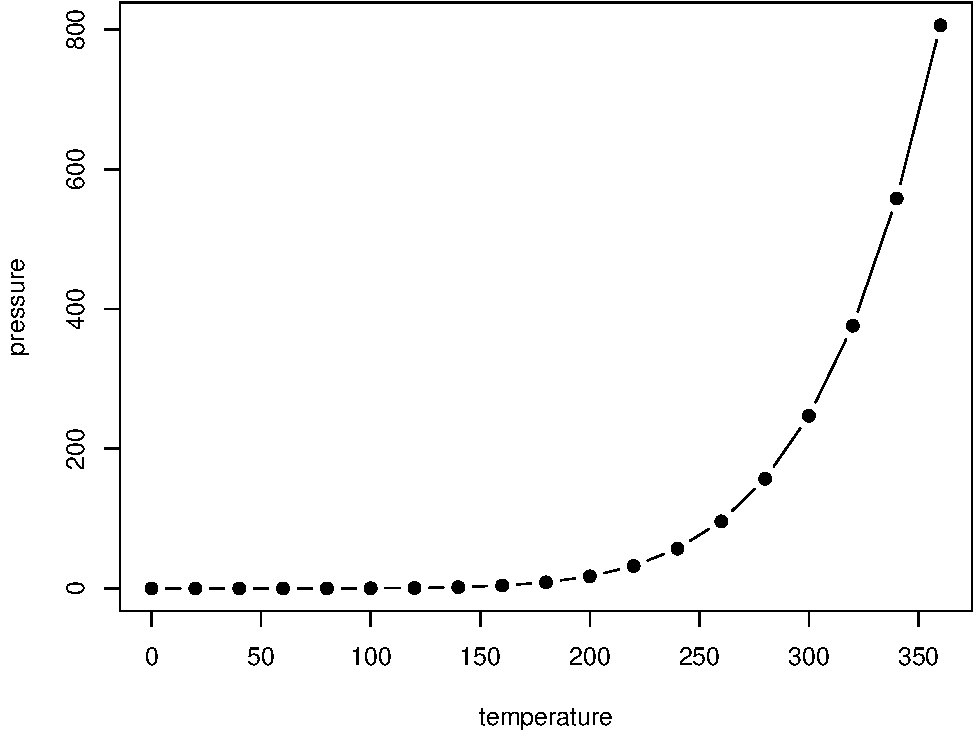
\includegraphics[width=0.8\linewidth]{_main_files/figure-latex/nice-fig-1} 

}

\caption{Here is a nice figure!}\label{fig:nice-fig}
\end{figure}

Don't miss Table \ref{tab:nice-tab}.

\begin{Shaded}
\begin{Highlighting}[]
\NormalTok{knitr}\SpecialCharTok{::}\FunctionTok{kable}\NormalTok{(}
  \FunctionTok{head}\NormalTok{(pressure, }\DecValTok{10}\NormalTok{), }\AttributeTok{caption =} \StringTok{\textquotesingle{}Here is a nice table!\textquotesingle{}}\NormalTok{,}
  \AttributeTok{booktabs =} \ConstantTok{TRUE}
\NormalTok{)}
\end{Highlighting}
\end{Shaded}

\begin{table}

\caption{\label{tab:nice-tab}Here is a nice table!}
\centering
\begin{tabular}[t]{rr}
\toprule
temperature & pressure\\
\midrule
0 & 0.0002\\
20 & 0.0012\\
40 & 0.0060\\
60 & 0.0300\\
80 & 0.0900\\
\addlinespace
100 & 0.2700\\
120 & 0.7500\\
140 & 1.8500\\
160 & 4.2000\\
180 & 8.8000\\
\bottomrule
\end{tabular}
\end{table}

\hypertarget{parts}{%
\chapter{Parts}\label{parts}}

You can add parts to organize one or more book chapters together. Parts can be inserted at the top of an .Rmd file, before the first-level chapter heading in that same file.

Add a numbered part: \texttt{\#\ (PART)\ Act\ one\ \{-\}} (followed by \texttt{\#\ A\ chapter})

Add an unnumbered part: \texttt{\#\ (PART\textbackslash{}*)\ Act\ one\ \{-\}} (followed by \texttt{\#\ A\ chapter})

Add an appendix as a special kind of un-numbered part: \texttt{\#\ (APPENDIX)\ Other\ stuff\ \{-\}} (followed by \texttt{\#\ A\ chapter}). Chapters in an appendix are prepended with letters instead of numbers.

\hypertarget{footnotes-and-citations}{%
\chapter{Footnotes and citations}\label{footnotes-and-citations}}

\hypertarget{footnotes}{%
\section{Footnotes}\label{footnotes}}

Footnotes are put inside the square brackets after a caret \texttt{\^{}{[}{]}}. Like this one \footnote{This is a footnote.}.

\hypertarget{citations}{%
\section{Citations}\label{citations}}

Reference items in your bibliography file(s) using \texttt{@key}.

For example, we are using the \textbf{bookdown} package \citep{R-bookdown} (check out the last code chunk in index.Rmd to see how this citation key was added) in this sample book, which was built on top of R Markdown and \textbf{knitr} \citep{xie2015} (this citation was added manually in an external file book.bib).
Note that the \texttt{.bib} files need to be listed in the index.Rmd with the YAML \texttt{bibliography} key.

The RStudio Visual Markdown Editor can also make it easier to insert citations: \url{https://rstudio.github.io/visual-markdown-editing/\#/citations}

\hypertarget{blocks}{%
\chapter{Blocks}\label{blocks}}

\hypertarget{equations}{%
\section{Equations}\label{equations}}

Here is an equation.

\begin{equation} 
  f\left(k\right) = \binom{n}{k} p^k\left(1-p\right)^{n-k}
  \label{eq:binom}
\end{equation}

You may refer to using \texttt{\textbackslash{}@ref(eq:binom)}, like see Equation \eqref{eq:binom}.

\hypertarget{theorems-and-proofs}{%
\section{Theorems and proofs}\label{theorems-and-proofs}}

Labeled theorems can be referenced in text using \texttt{\textbackslash{}@ref(thm:tri)}, for example, check out this smart theorem \ref{thm:tri}.

\begin{theorem}
\protect\hypertarget{thm:tri}{}\label{thm:tri}For a right triangle, if \(c\) denotes the \emph{length} of the hypotenuse
and \(a\) and \(b\) denote the lengths of the \textbf{other} two sides, we have
\[a^2 + b^2 = c^2\]
\end{theorem}

Read more here \url{https://bookdown.org/yihui/bookdown/markdown-extensions-by-bookdown.html}.

\hypertarget{callout-blocks}{%
\section{Callout blocks}\label{callout-blocks}}

The R Markdown Cookbook provides more help on how to use custom blocks to design your own callouts: \url{https://bookdown.org/yihui/rmarkdown-cookbook/custom-blocks.html}

\hypertarget{sharing-your-book}{%
\chapter{Sharing your book}\label{sharing-your-book}}

\hypertarget{publishing}{%
\section{Publishing}\label{publishing}}

HTML books can be published online, see: \url{https://bookdown.org/yihui/bookdown/publishing.html}

\hypertarget{pages}{%
\section{404 pages}\label{pages}}

By default, users will be directed to a 404 page if they try to access a webpage that cannot be found. If you'd like to customize your 404 page instead of using the default, you may add either a \texttt{\_404.Rmd} or \texttt{\_404.md} file to your project root and use code and/or Markdown syntax.

\hypertarget{metadata-for-sharing}{%
\section{Metadata for sharing}\label{metadata-for-sharing}}

Bookdown HTML books will provide HTML metadata for social sharing on platforms like Twitter, Facebook, and LinkedIn, using information you provide in the \texttt{index.Rmd} YAML. To setup, set the \texttt{url} for your book and the path to your \texttt{cover-image} file. Your book's \texttt{title} and \texttt{description} are also used.

This \texttt{gitbook} uses the same social sharing data across all chapters in your book- all links shared will look the same.

Specify your book's source repository on GitHub using the \texttt{edit} key under the configuration options in the \texttt{\_output.yml} file, which allows users to suggest an edit by linking to a chapter's source file.

Read more about the features of this output format here:

\url{https://pkgs.rstudio.com/bookdown/reference/gitbook.html}

Or use:

\begin{Shaded}
\begin{Highlighting}[]
\NormalTok{?bookdown}\SpecialCharTok{::}\NormalTok{gitbook}
\end{Highlighting}
\end{Shaded}


  \bibliography{book.bib,packages.bib}

\end{document}
